\documentclass{article}
\usepackage[margin=2cm]{geometry}
\usepackage{graphicx}
\usepackage{hyperref}

\title{Snake: Developer Guide}
\author{Alessandra Sasanelli, Simone Maccario}
\date{\today}

\begin{document}
	\maketitle
	\abstract{
		This document is meant to show the source code of the project. 
		After giving a brief overview on the structure of the project, the libraries used and how are the code is divided between the files, 
		it will illustrate all of the main functions.
	}
	
	\section{The structure of the project}
	The folder of the main project contains 3 subdirectories: 
	\begin{itemize}
		\item docs is meant to hold all of the non-relevant to code files, like the README.txt, the proposal and the two guides
		\item resources is used to hold all of the images and sounds used by the game: into the images folder there are all of the images; into the sounds folder there are all of the sounds, whilst in the numbers folder, there are the images of the numbers (used to track the user score)
		\item code holds all of the source files for the project; inside, the subdirectory external-files has all of the auxiliary code files
	\end{itemize}
	
	\section{The libraries}	
	This project uses three main libraries:
	\begin{itemize}
		\item \textbf{racket/base} --$>$ used to import and export functions, structures and constants from file to file 
		(\href{https://docs.racket-lang.org/reference/index.html}{documentation})
		\item \textbf{2htdp/universe} --$>$ used to make the interactive application thanks to the provided big-bang function 
		(\href{https://docs.racket-lang.org/teachpack/2htdpuniverse.html}{documentation})
		\item \textbf{2htdp/image} --$>$ used to render the application. From this library, we imported also racket/gui/base play-sound (\href{https://docs.racket-lang.org/gui/Windowing_Functions.html#\%28def._\%28\%28lib._mred\%2Fmain..rkt\%29._play-sound\%29\%29}{documentation of the function here}) function 	
		(\href{https://docs.racket-lang.org/teachpack/2htdpimage.html}{documentation})
	\end{itemize}
	
	\pagebreak
	
	\section{Source code}
	This section will discuss the main functions developed to make the application. It will focus on every single file to explain the functions present in each of them.
	
	\subsection{positions.rkt}
	This file contains all the functions relative to the positions; below, are listed and explained a few of them.
	Here won't be listed all simple auxiliary functions, which are: increment-pos, decrement-pos, direction-by-posn, delete-el.
	\begin{itemize}
		\item \textbf{make-positions}: \\
			\emph{signature}: Number Number Number List$<$Posn$>$ -$>$ List$<$Posn$>$ \\
			\emph{purpose}: computes all the positions on the background before the game starts \\
			\emph{explanation}: this function has four parameters: `n` (the starting position count), `x` and `y` (initial row and column), and a list of existing positions. To map positions on a 501x501 pixel background, where each position spans 25x25 pixels, use parameters 1, 1, 1, and `(list (make-posn 13 13))`. The recursion halts at `n = 400`, the maximum positions possible on this background, marking the base case. If a row is filled, increase `n` and `y` to move to the next row. Otherwise, increment `n` and `x` for the next column. Each position, determined by row and column, is added to the positions list.
			\begin{figure}[h!]
				\centering
				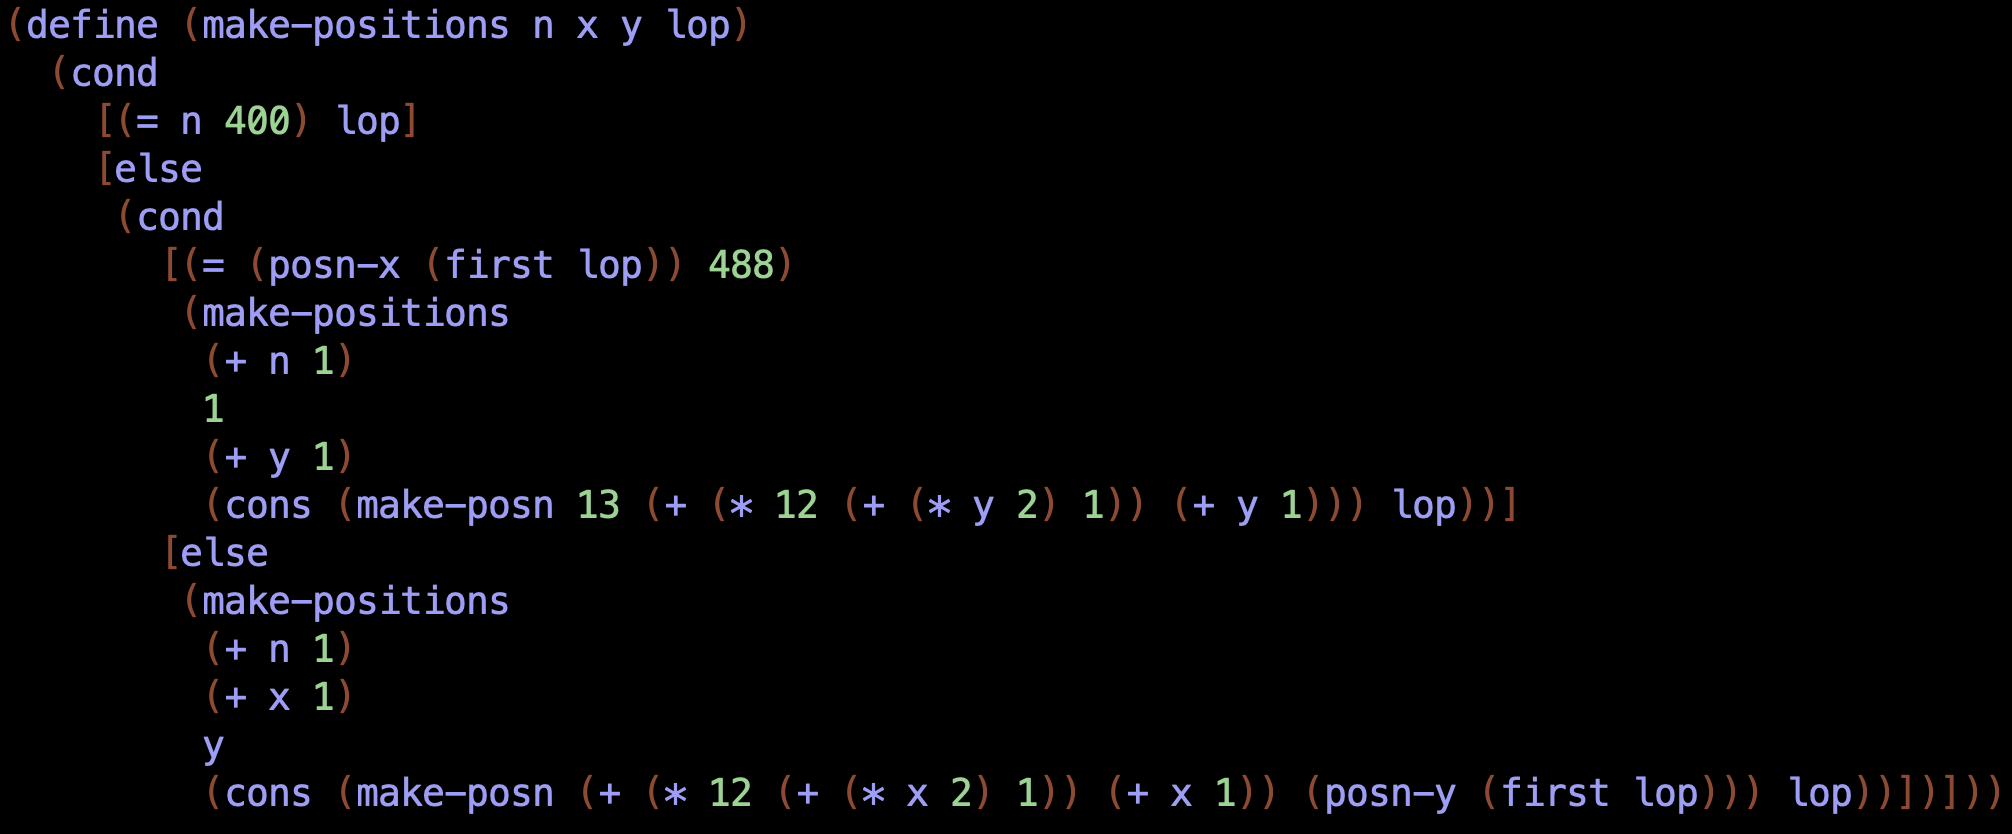
\includegraphics[width=.6\linewidth]{make-position.png}
				\caption{make-position function in racket}
			\end{figure}
			
		\item \textbf{compute-available-pos}: \\
			\emph{signature}: List$<$Posn$>$ List$<$Posn$>$ -$>$ List$<$Posn$>$ \\
			\emph{purpose}: computes available positions on the background \\
			\emph{explanation}: this function performs recursion over two lists: `lop-snake`, which holds positions of the snake to be removed from the available positions in `lop`. The base case occurs when either or both lists are empty, indicating all positions have been evaluated and are unoccupied, so `lop` is returned. Otherwise, the function recursively processes the remainder of `lop-snake` and applies `delete-el` to the first element of `lop-snake` and the `lop` list. The `delete-el` function either retains `lop` as is or removes an element from it if it matches the first element of `lop-snake`.
			\begin{figure}[h!]
				\centering
				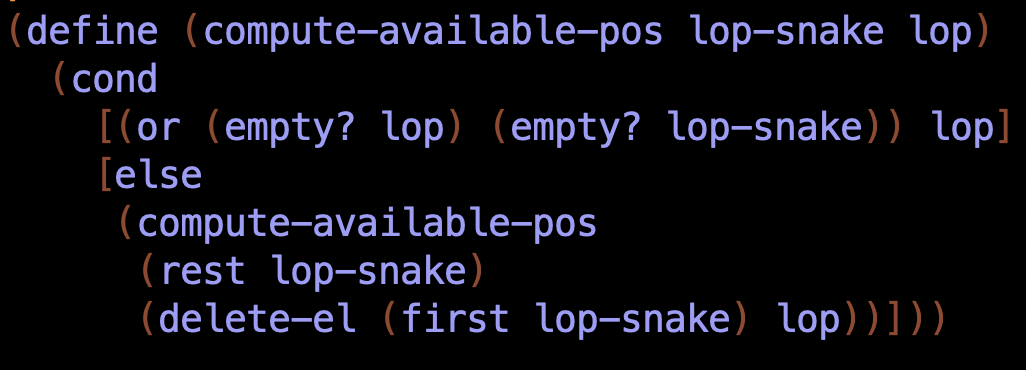
\includegraphics[width=.6\linewidth]{compute-available-pos.png}
				\caption{compute-available-pos function in racket}
			\end{figure}
			
		\item \textbf{compute-apple-position}: \\
			\emph{signature}: Number Number List$<$Posn$>$ -$>$ Apple \\
			\emph{purpose}: computes all the positions on the background before the game starts \\
			\emph{explanation}: this function has three parameters, including an accumulator. It selects a position from available positions using `n`, which ranges from 1 (inclusive) to 401 (exclusive). The base case triggers if the list is empty or `n` equals the accumulator, returning the first element. Otherwise, it recurses over the rest of the list, incrementing the accumulator by one.
			\begin{figure}[h!]
				\centering
				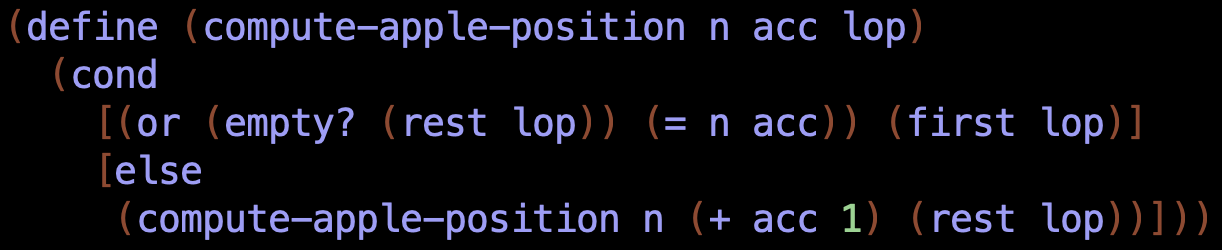
\includegraphics[width=.6\linewidth]{compute-apple-position.png}
				\caption{compute-apple-position function in racket}
			\end{figure}
			
		\item \textbf{check-position-out}: \\
			\emph{signature}: Posn List$<$Posn$>$ -$>$ Boolean \\
			\emph{purpose}: checks wheather the given posn is into backgroundpos \\
			\emph{explanation}: in the base case, if the list is empty, the list returns true. 
							The other case happens if the first element of the list is equal to pos; at this point, the function returns 								false.
							In the recursive case, we simply call the function again on the rest of the list.
			\begin{figure}[h!]
				\centering
				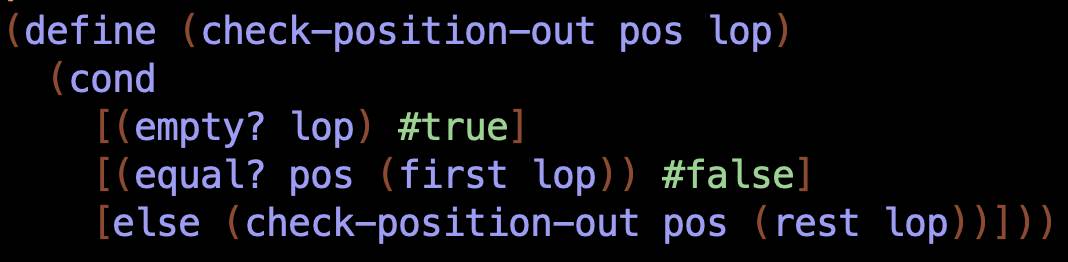
\includegraphics[width=.6\linewidth]{check-position-out.png}
				\caption{check-position-out function in racket}
			\end{figure}
			
		\item \textbf{update-positions}: \\
			\emph{signature}: Direction List$<$Posn$>$ -$>$ List$<$Posn$>$ \\
			\emph{purpose}: updates a list of positions based on itself and the head direction \\
			\emph{explanation}: this function processes a list of `posn` and outputs a new list with updated `posn` based on a given direction. The base case occurs when only one `posn` remains in the list, which is then updated according to the `direction` field in the `snake` structure. In the recursive case, the function constructs a list by applying `compute-new-posn` to the first list element. This function generates a new `posn` based on the direction determined by both the current and next `posn` in the list.
			\begin{figure}[h!]
				\centering
				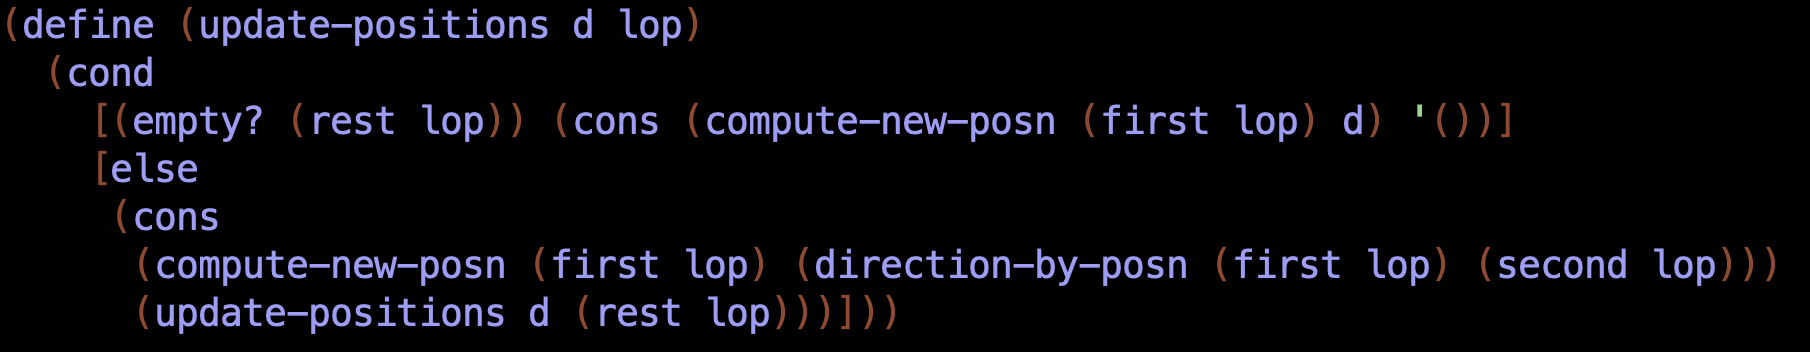
\includegraphics[width=.6\linewidth]{update-positions.png}
				\caption{update-positions function in racket}
			\end{figure}
	\end{itemize}
	
	\pagebreak
	
	\subsection{snake.rkt}
	This file contains all the functions relative to the snake. Of all the functions written, it is only shown the main one, the draw-snake. The others are: change-snake-direction, which simply returns a snake with changed direction based on the direction inputed, move-snake which return a snake but calling the update-positions on the snake-position, check-eat-snake which simply returns true if the position of the head is equal to any other into the snake-position.
	\begin{itemize}
		\item \textbf{draw-snake}: \\
			\emph{signature}: Snake -$>$ Image \\
			\emph{purpose}: draws the snake on the background \\
			\emph{explanation}: in this function for drawing a snake in the graphical interface, different conditions are applied in recursion to handle the head, tail, and body units of the snake. The base case occurs when there's only one element left in the list, indicating the head of the snake, which is then placed and rotated on the background based on its direction using `rotate-el`. When the list's length is equal to the snake's length, the function identifies it as the tail to be drawn, applying `rotate-el` for rotation, with its direction influenced by the tail itself and the subsequent element. In the recursive case, `place-image` is used for the first element of the list, drawing a snake unit at the specified position. This process is repeated for the remaining list, thereby drawing each body unit of the snake.
			\begin{figure}[h!]
				\centering
				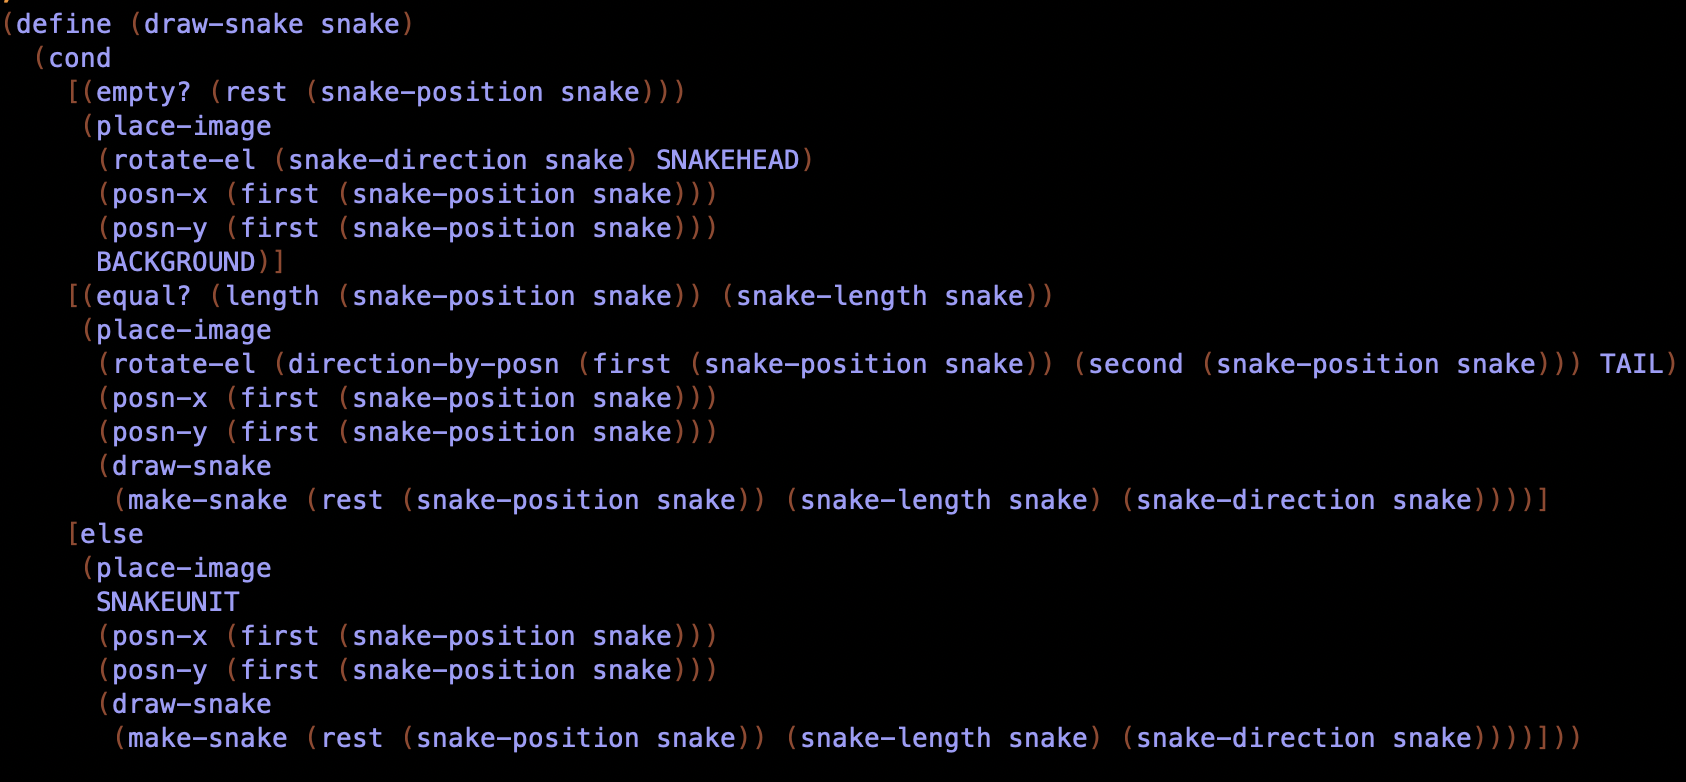
\includegraphics[width=.6\linewidth]{draw-snake.png}
				\caption{draw-snake function in racket}
			\end{figure}
	\end{itemize}
	
	\subsection{generals.rkt}
	This file contains all the functions that are of general purpose. This file mainly provides constants, but it also provides two functions, one of which will be explained here. One important constant is the NUMBERS, which is a list containing the paths to the images of the single numbers.
	\begin{itemize}
		\item \textbf{number-$>$image}: \\
			\emph{signature}: StringOfNumbers Number -$>$ Image \\
			\emph{purpose}: takes in a number and returns it as an image \\
			\emph{explanation}: the number n represents the initial indices of the character in the string of numbers. So, the base case will be when n-1 is equal to the string length. In this case, we just call the bitmap/file function on the path of the file, which gets returned by the function number-$>$path. The recursive case simply calls the beside function on the element of the string at index n and on the recursive call on the function with the same string and n incremented by one.
			\begin{figure}[h!]
				\centering
				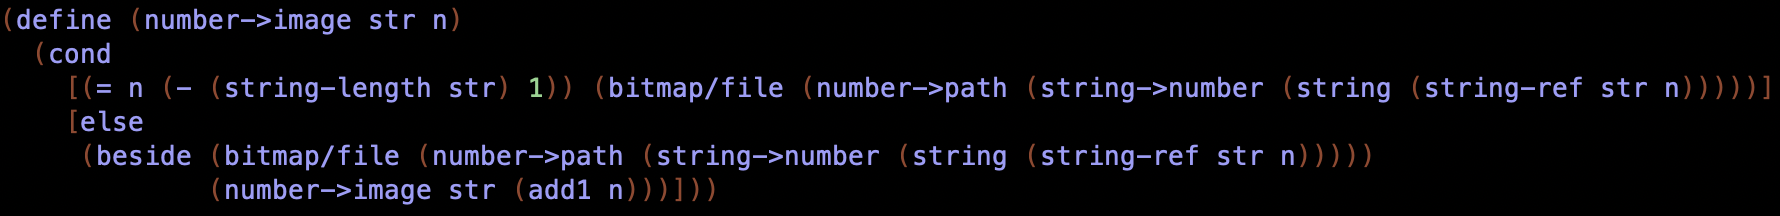
\includegraphics[width=.6\linewidth]{number-image.png}
				\caption{number-image function in racket}
			\end{figure}
	\end{itemize}
	
	\pagebreak
	
	\subsection{snake-final.rkt}
	This file contains all the functions that are needed to make the big-bang work. Most of these functions take in an Appstate.
	\begin{itemize}
		\item \textbf{handle-keyboard}: \\
			\emph{signature}: AppState KeyboardEvent -$>$ AppState \\
			\emph{purpose}: handles the keyboard events \\
			\emph{explanation}: this function is a big conditional that checks the string KeyboardEvent. If the key pressed is "s", then we call the start function, which simply sets the game field to true. The second condition check if the key arrow pressed is opposite to the direction the snake head had previously to block the operation. If "r" is pressed, the function calls the reset function, which simply returns the default appstate. The "escape" key changes the quit field to true, making the app quitting and closing right after. For every other case, the function simply returns the given state.
			\begin{figure}[h!]
				\centering
				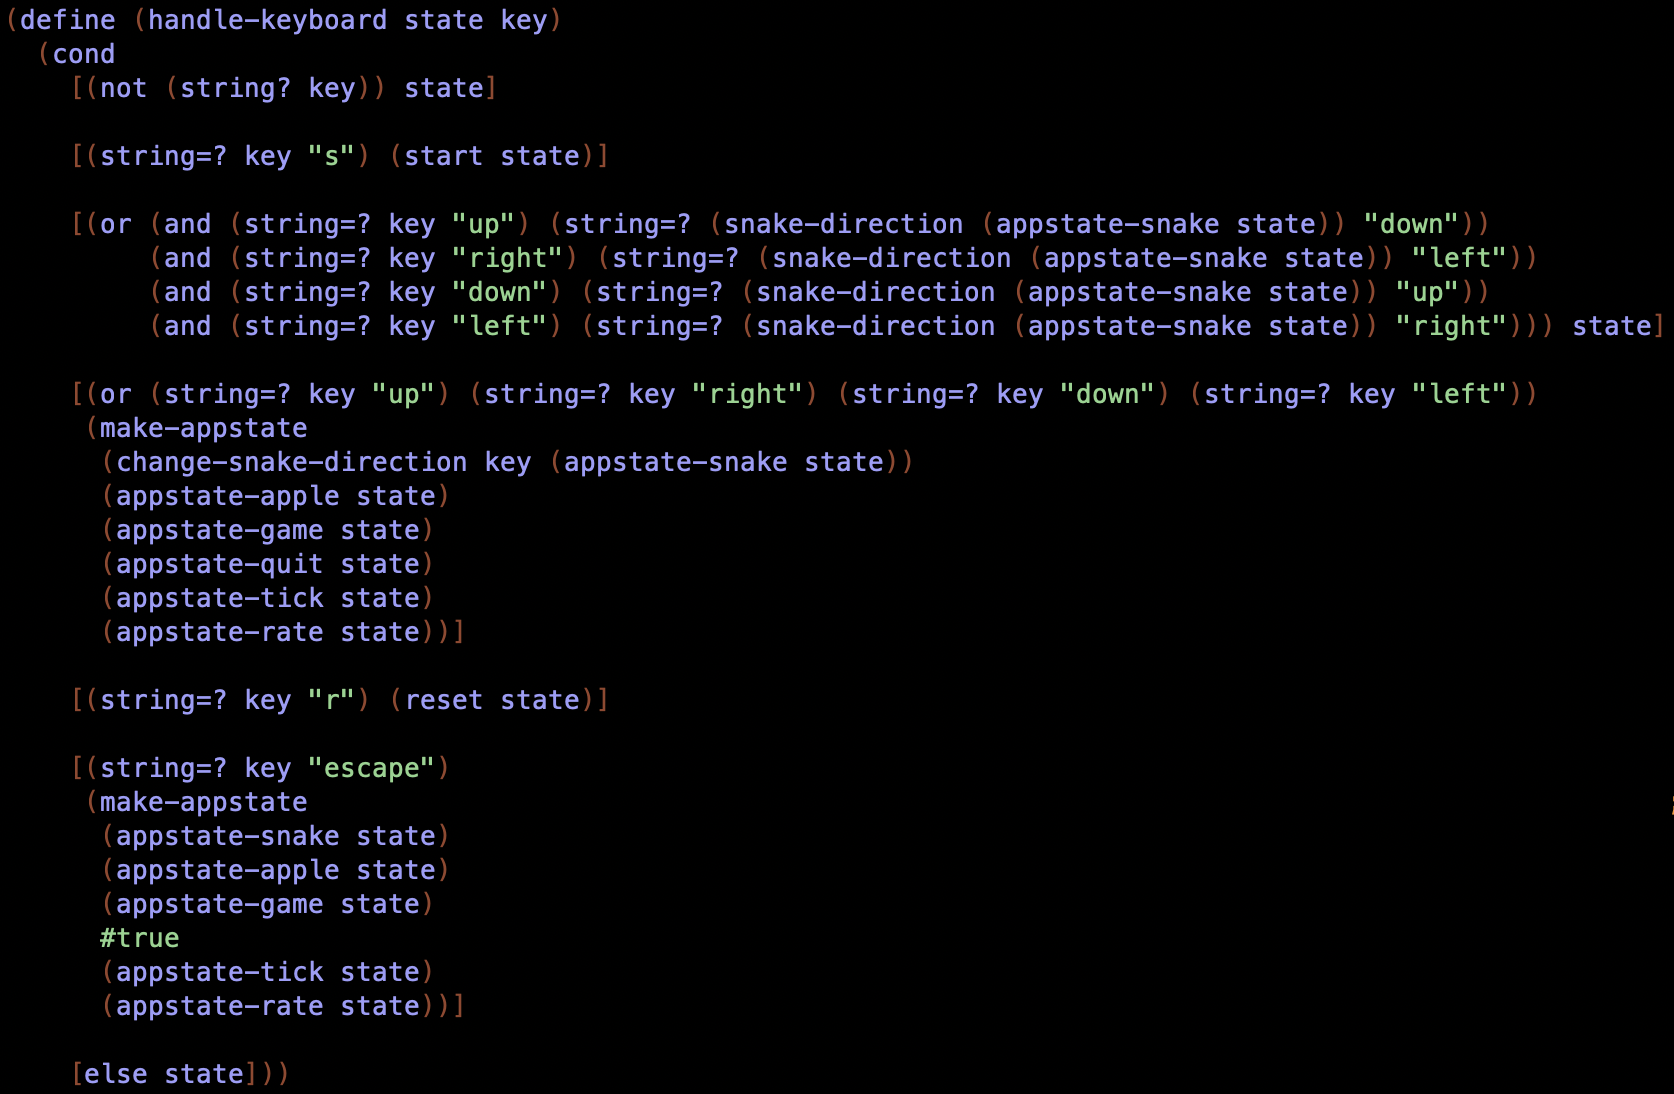
\includegraphics[width=.6\linewidth]{handle-keyboard.png}
				\caption{handle-keyboard function in racket}
			\end{figure}
			
		\item \textbf{eating}: \\
			\emph{signature}: AppState -$>$ AppState \\
			\emph{purpose}: handles the eating event of the game \\
			\emph{explanation}: when the function is called, it first plays a sound. The main operation involves creating a new `appstate` with an updated snake, which is moved using `move-snake`. This updated snake has a new position added to its `snake-position` field, and its length is increased by one. Next, the apple's position is recalculated using `compute-apple-pos`, which takes a list of snake positions, the previous apple position, and all background positions. Finally, the `rate` field is reduced by one only after three apples have been eaten.
			\begin{figure}[h!]
				\centering
				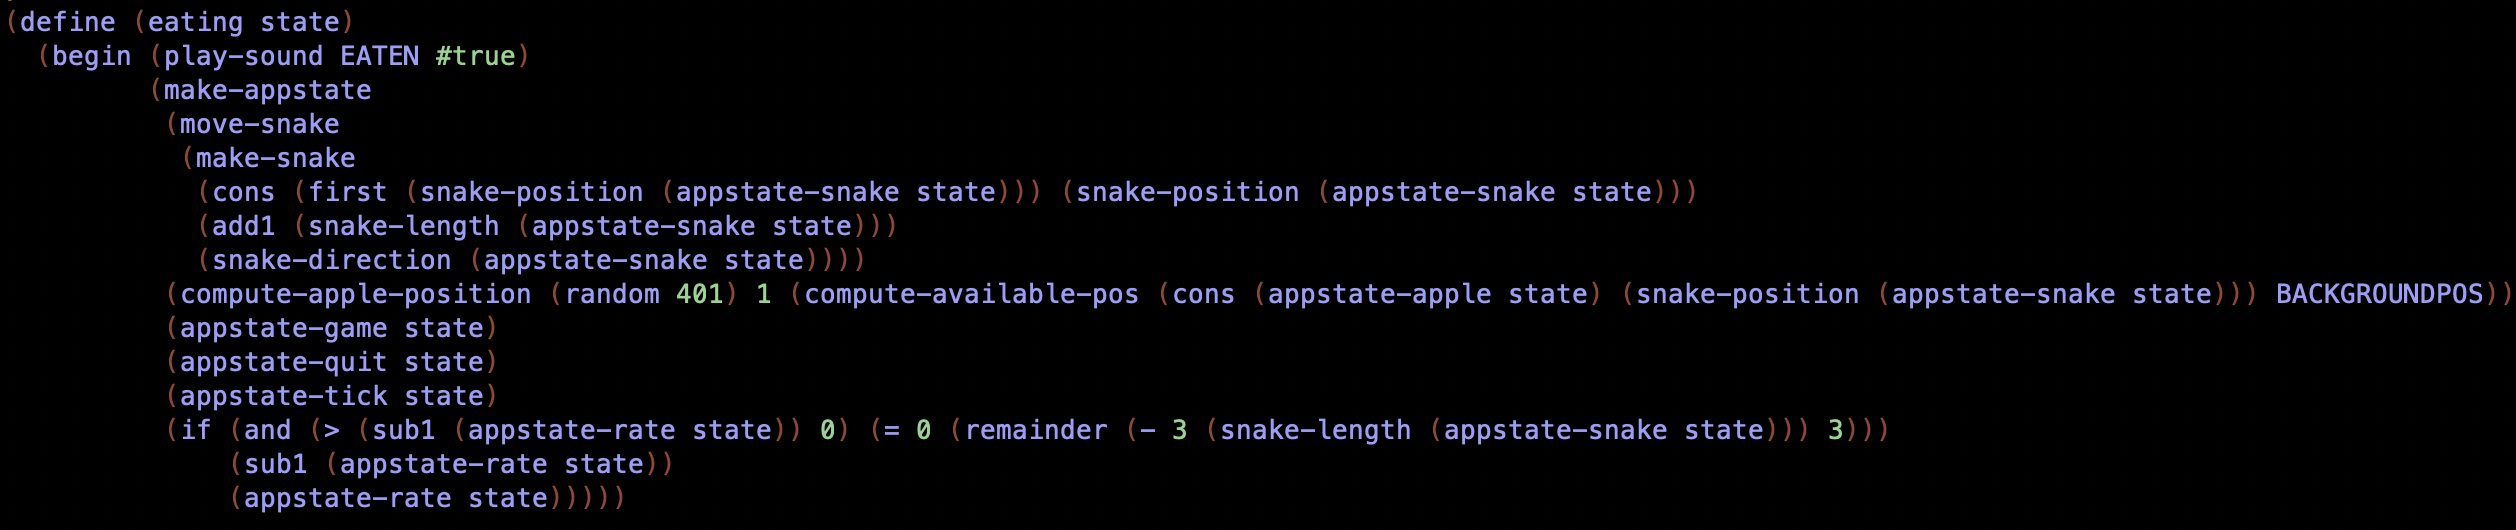
\includegraphics[width=.6\linewidth]{eating.png}
				\caption{eating function in racket}
			\end{figure}
			
		\item \textbf{move}: \\
			\emph{signature}: AppState -$>$ AppState \\
			\emph{purpose}: used to change the appstate on tick \\
			\emph{explanation}: if the end condition is met on tick, the game and quit fields are set to false. If `appstate` game is false, the function returns the unchanged `appstate`. The function then checks the remainder of tick divided by rate, with tick counting clock ticks since start and rate indicating speed levels. If the remainder is zero, `appstate` is updated either by moving the snake or calling the eating function, making the snake faster as rate decreases. If none of these conditions are met, `appstate` is returned with the tick field incremented by one.
			\begin{figure}[h!]
				\centering
				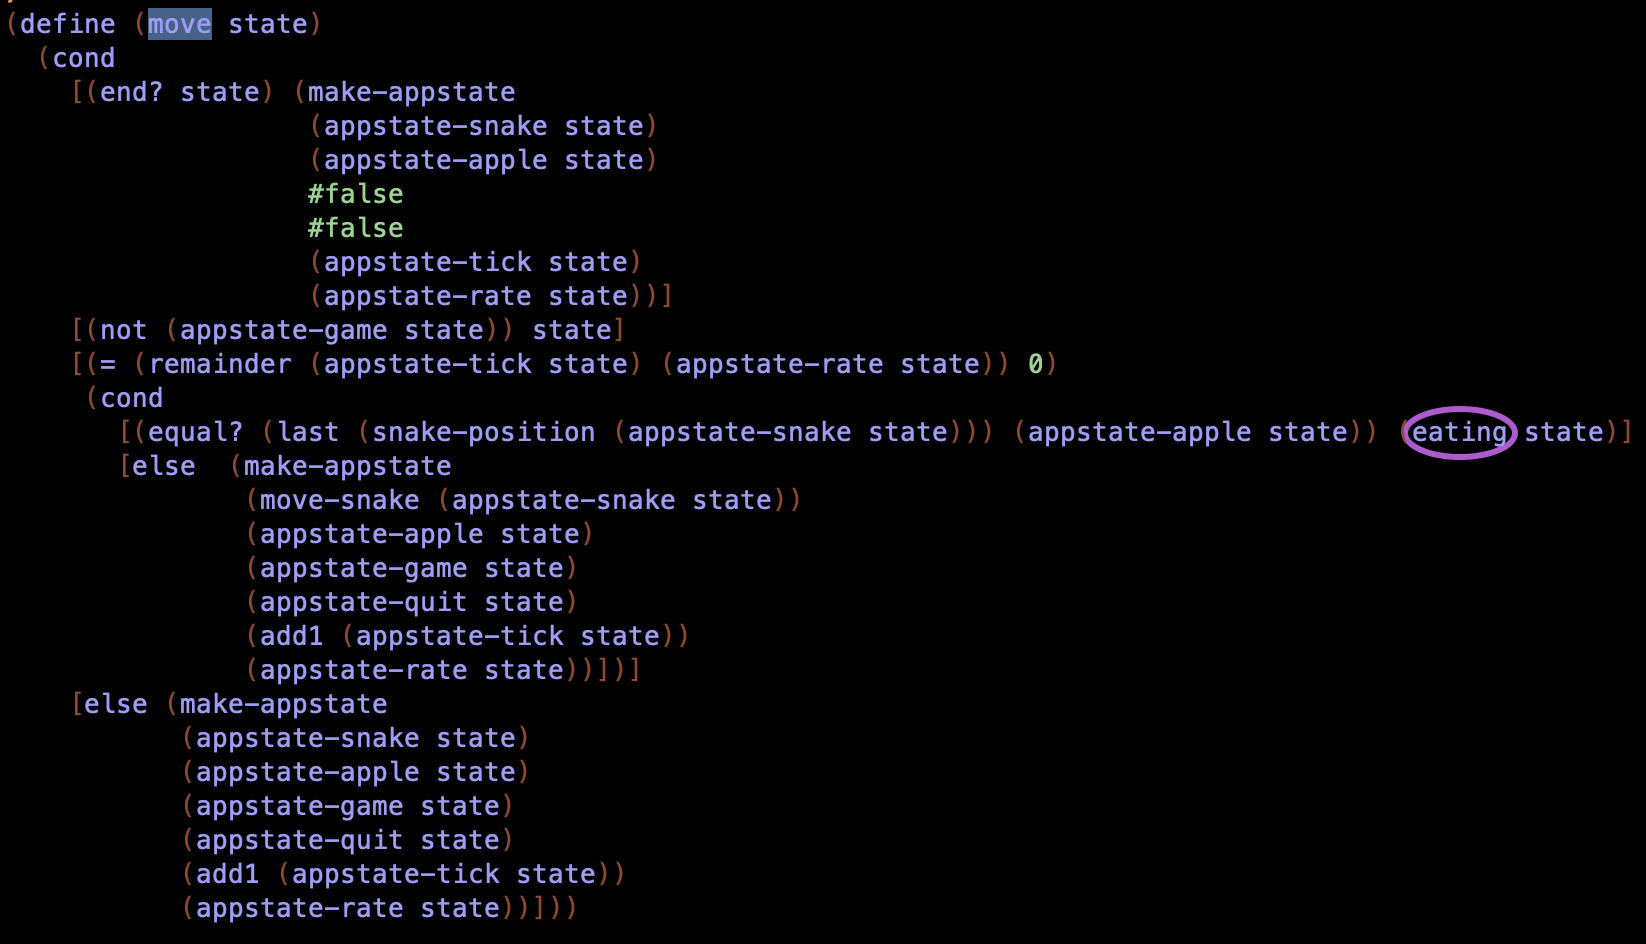
\includegraphics[width=.6\linewidth]{move.png}
				\caption{move function in racket}
			\end{figure}
			
		\item \textbf{end?}: \\
			\emph{signature}: AppState -$>$ Boolean \\
			\emph{purpose}: checks weather the game is in gameover or not \\
			\emph{explanation}: it simply checks whether the snake has gone over the borders of the game or if it has eaten itself. Then, if this condition is true, the function returns true and plays the game over sound, setting the GAMEOVRPLAYED to true. Otherwise, it resets GAMAOVRPLAYED to false and return false.
			\begin{figure}[h!]
				\centering
				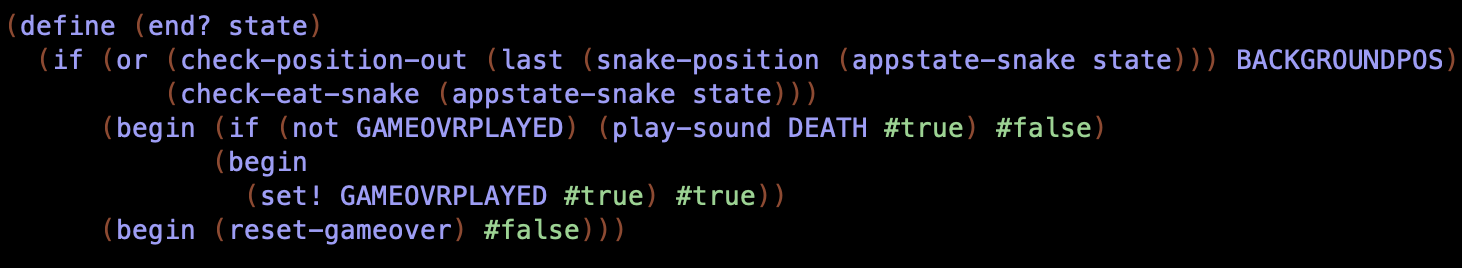
\includegraphics[width=.6\linewidth]{end.png}
				\caption{end? function in racket}
			\end{figure}
	\end{itemize}

\end{document}